\chapter{Result }
\label{ch:intro}

\section{Experimental Environment}

\subsection{Hardware Setup}
All experiments were conducted on a Laptop machine equipped with an Intel\textsuperscript{\textregistered} Core\textsuperscript{TM} i7 CPU (details of clock speed can be added) and 32\,GB of RAM , as well as on a mobile \emph{Hunter} robotic platform for on-campus data collection. The Hunter robot is equipped with:
\begin{itemize}
    \item A LiDAR sensor,
    \item An IMU (for attitude and acceleration),
    \item A camera
    \item An onboard NVIDIA CPU/GPU module for local processing.
\end{itemize}
Data were stored on a standard SSD. This configuration proved sufficient to process LiDAR scans at real-time rates, especially when selectively loading sub-maps.

\subsection{Software Setup}
Our approach is implemented primarily in C++ on top of the ROS\,2 Humble middleware. We rely on:
\begin{itemize}
  \item \textbf{PCL (Point Cloud Library):} for point cloud data structures and filtering.
  \item \textbf{Eigen:} for linear algebra operations (transformations, matrix computations).
  \item \textbf{ROS\,2 Bag Files:} each dataset is provided or recorded in a \texttt{.bag} format, facilitating playback of sensor data.
\end{itemize}
Additional scripts in Python were employed for plotting and minor data manipulations.

\subsection{Datasets}
We evaluated our map-based localization on multiple datasets, each of which offers LiDAR and IMU data. Table~\ref{tab:datasets} summarizes their key characteristics.

\begin{table}[htbp]
\centering
\caption{Overview of datasets and sensor configurations. (L: LiDAR; I: IMU)}
\label{tab:datasets}
\resizebox{\textwidth}{!}{%
\begin{tabular}{lccccc}
\toprule
\textbf{Dataset} & \textbf{Seq.} & \textbf{Sensors} & \textbf{LiDAR Type} & \textbf{Frequencies (Hz)} & \textbf{Map Prep. Method} \\
\midrule
\textbf{KITTI Odometry} & 05 & L + I & Velodyne HDL-64E & L: 10, I: 100 & GT-based aggregation \\
%\textbf{KITTI Odometry} & 09 & L + I & Velodyne HDL-64E & L: 10, I: 100 & GT-based aggregation \\
\textbf{MulRan}         & KiAST-02 & L + I & Ouster OS1-64    & L: 10, I: 100 & Fast-LIO2 SLAM \\
\textbf{MulRan}         & KiAST-03 & L + I & Ouster OS1-64    & L: 10, I: 100 & Fast-LIO2 SLAM \\
\textbf{Saxion campus}  & seq1 & L + I & Ouster OS1-128    & L: 10, I: 100 & Fast-LIO2 SLAM \\

%\bottomrule
%\end{tabular}%
%}
%\end{table}

\paragraph{KITTI Sequences}
We tested on sequences 05 from the KITTI odometry benchmark. These sequences contain semi-urban driving scenarios with moderate speeds. Each frame is timestamped and stored in a ROS\,2 bag for convenient playback.

\paragraph{MulRan (KiAST) Sequences}
Two sequences (KiAST-02, KiAST-03) from the MulRan dataset were used. These contain Ouster OS1-64 LiDAR and IMU measurements in campus-like settings with dynamic objects and complex geometry. The ROS\,2 bags allow consistent replay for algorithm testing.

\subsection{Map Preparation}
For each dataset, a prior 3D map was generated before running the localization:

\begin{itemize}
    \item \textbf{KITTI:} We leveraged the official ground-truth poses to transform and aggregate each LiDAR frame into a global coordinate system. The resulting dense point cloud was lightly downsampled (e.g., voxel size of 0.1\,m).
    \item \textbf{MulRan (KiAST) and Campus (Saxion) Dataset:} No direct ground truth was provided, so we employed \textit{Fast-LIO2 SLAM} to build a consistent map from repeated traversals. This method fuses LiDAR scans and IMU data for robust odometry. The final aggregated map was also voxel-downsampled.
\end{itemize}

In both cases, the final global point cloud is subdivided into manageable tiles (e.g., 50\,m $\times$ 50\,m in the XY-plane) for efficient dynamic loading during localization. Each tile is stored as a separate file or database entry keyed by tile coordinates, allowing the system to load only relevant tiles based on the vehicle’s current estimated position.

Overall, this setup ensures that the offline map is readily available in a lightweight format, and the runtime memory footprint remains controlled as the vehicle traverses large-scale environments.


% \section{Result}

% \subsection{Dynamic Map Loading}
% Dynamic map loading is implemented to optimize memory and computational efficiency in large-scale localization. Instead of loading the entire map, only the relevant portion is loaded dynamically based on the robot’s current position. This method significantly reduces memory consumption and improves real-time performance.
% The following images from **RViz** illustrate the dynamic map loading process. The **active map region** is highlighted in red colors, showing how the system loads only necessary portions as the robot moves.

% \begin{figure}[h]
%     \centering
%     \begin{subfigure}{0.49\textwidth}
%         \includegraphics[width=\linewidth]{images/kitti_load2.png}
%         \caption{Initial Map Loading}
%     \end{subfigure}
%     \hfill
%     \begin{subfigure}{0.49\textwidth}
%         \includegraphics[width=\linewidth]{images/kitti_load1.png}
%         \caption{Map Updated as Robot Moves}
%     \end{subfigure}
    
%     % \begin{subfigure}{0.45\textwidth}
%     %     \includegraphics[width=\linewidth]{map_loading_3.png}
%     %     \caption{Further Update in a New Region}
%     % \end{subfigure}
%     % \hfill
%     % \begin{subfigure}{0.45\textwidth}
%     %     \includegraphics[width=\linewidth]{map_loading_4.png}
%     %     \caption{Final State: Only Active Regions are Loaded}
%     % \end{subfigure}
    
%     \caption{RViz Visualization of Dynamic Map Loading. The red region represents the currently loaded map section and the green color shows current LIDAR scan}
%     \label{fig:dynamic_map_loading}
% \end{figure}

% \subsection{NDT  Localization Result}


% \paragraph{NDT scan and map alignment }
% Figure \ref{fig:ndt_allignment} show the NDT registration visualization in saxion campus dataset.
% \begin{figure}[h]
%     \centering
%     \begin{subfigure}{0.49\textwidth}
%         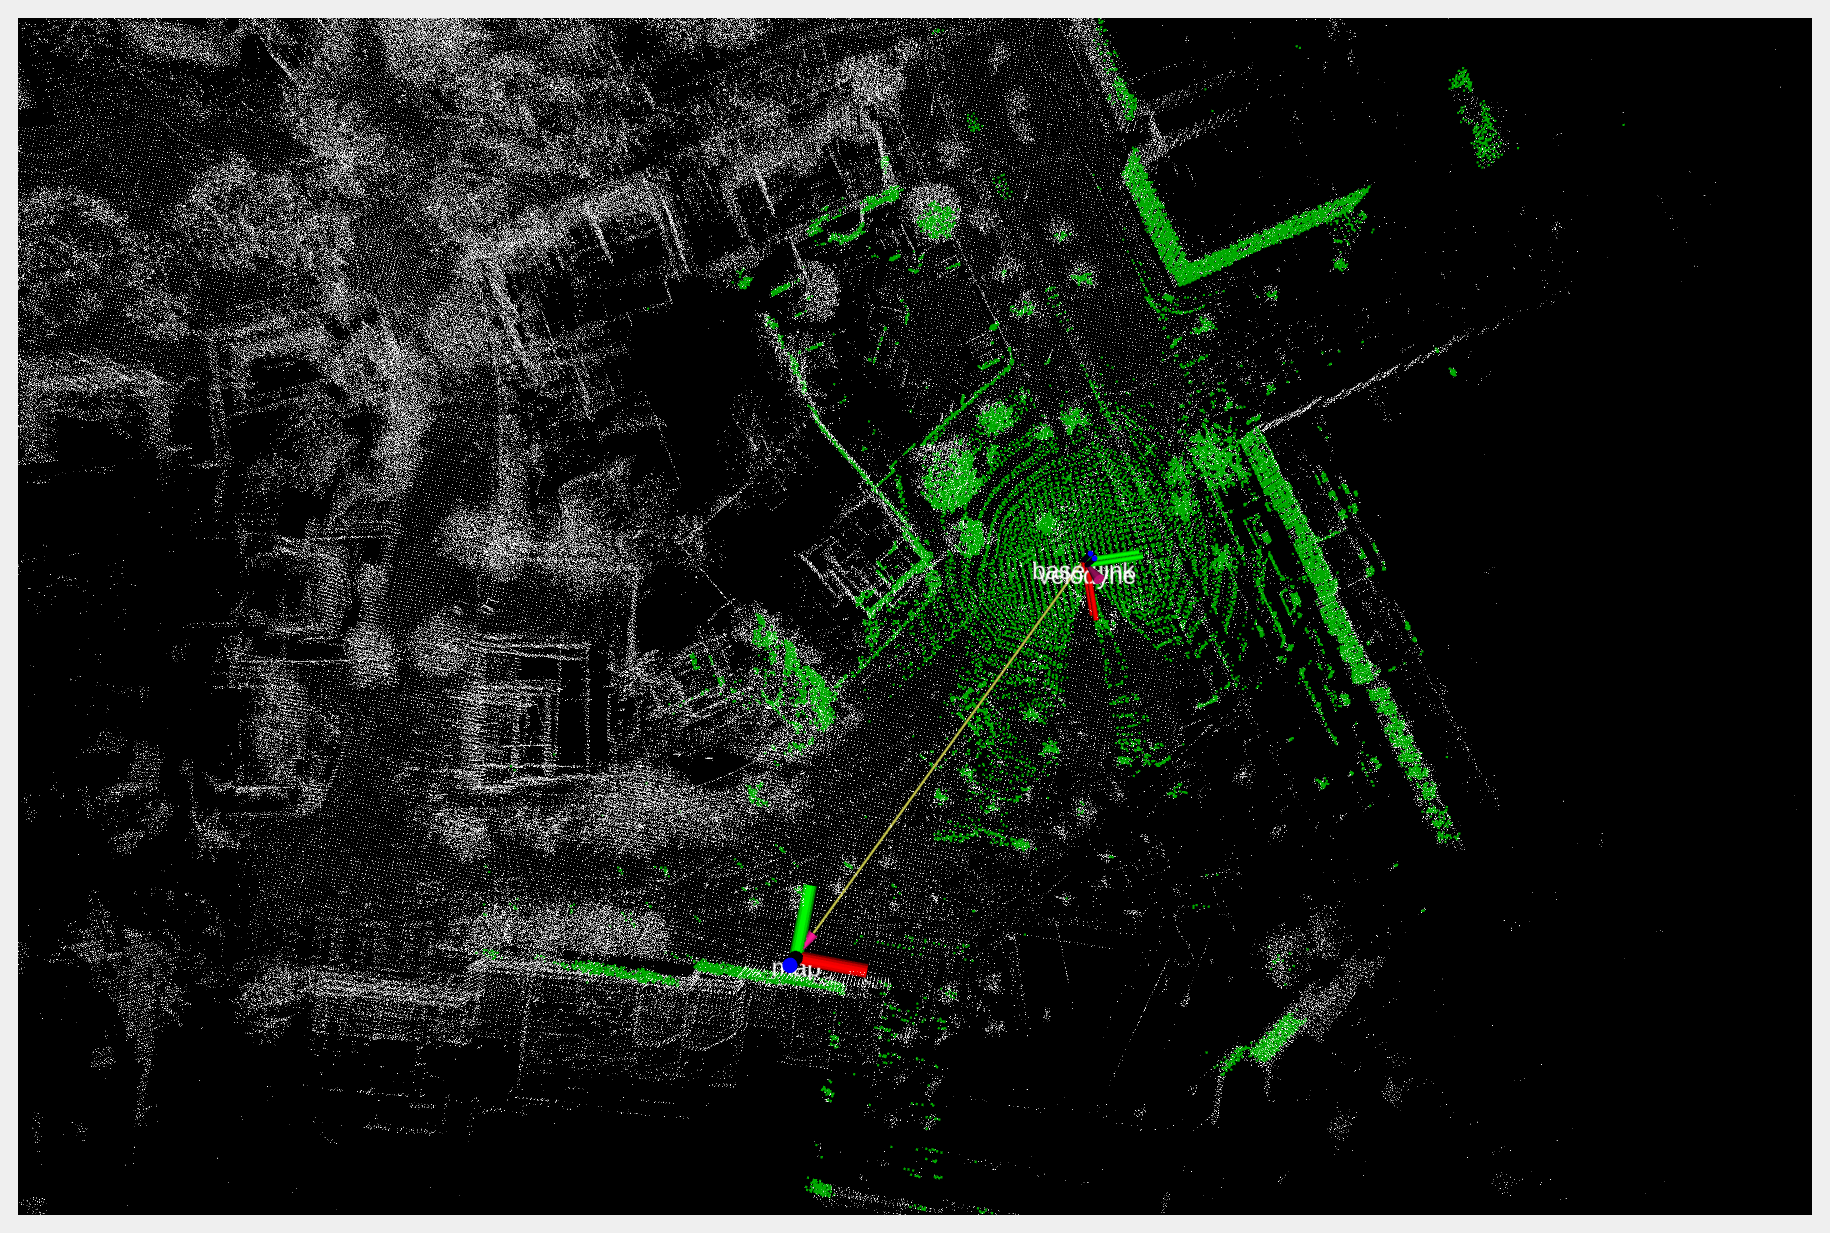
\includegraphics[width=\linewidth]{images/ndt_scan_map_matching2.png}
%         \caption{Initial Map Loading}
%     \end{subfigure}
%     \hfill
%     \begin{subfigure}{0.49\textwidth}
%         \includegraphics[width=\linewidth]{images/ndt_scan_map_matching.png}
%         \caption{Map Updated as Robot Moves}
%     \end{subfigure}
%     \caption{RViz Visualization of current scan with map allignment using NDT registration. The green color scan represents the currently scan and the greycolor  color shows global map}
%     \label{fig:ndt_allignment}
% \end{figure}


% \paragraph{KITTI Sequence 5 Test}
% Multiple runs of NDT localization on KITTI Sequence 5 revealed cases where localization either succeeded or failed. Below, we present separate images for these scenarios.

% \begin{itemize}
%     \item As shown in Figure \ref{fig:kitti_fail}, localization failure occurs in certain sections of the trajectory.
%     \begin{figure}[ht]
%     \centering
%     \includegraphics[width=0.6\textwidth]{images/kitti_failure.png}
%     \caption{Example of NDT localization failure in KITTI Sequence 5.}
%     \label{fig:kitti_fail}
%     \end{figure}

%     \item Figure \ref{fig:kitti_success} shows a scenario where localization performs well. The robot finishes the whole trajectory.
%     \begin{figure}[ht]
%     \centering
%     \includegraphics[width=0.6\textwidth]{images/kitti_suces.png}
%     \caption{Successful NDT localization in KITTI Sequence 5.}
%     \label{fig:kitti_success}
%     \end{figure}

% \end{itemize}

% \paragraph{Saxion Dataset Test}

% \begin{figure}[ht]
%     \centering
%     \includegraphics[width=0.6\textwidth]{images/saxionfailure.png}
%     \caption{Example of NDT localization failure in the Saxion dataset.}
%     \label{fig:saxion_fail}
% \end{figure}

% In Figure \ref{fig:saxion_fail}, NDT localization fails in certain regions of the Saxion dataset.


% \subsubsection{Things to be Checked for Localization failure }
% \begin{itemize}
%     \item NDT registration parameters 
%     \item Map and Scan down-sampling parameter 
%     \item Map Retrial radius 
%     \item Map Quality 
% \end{itemize}
